\documentclass[11pt,twoside]{book}
\usepackage{times,mathptm,multirow,fancyvrb,color}
%\usepackage{picins}

%\usepackage{wrapfig}
\usepackage[pdftex]{graphicx}
\usepackage{hyperref}
\pdfcompresslevel=9
\DeclareGraphicsExtensions{.jpg,.pdf,.png}
\usepackage{setspace,moreverb}

\usepackage{color}

\pagestyle{plain}

\setlength{\textwidth}{6.5in}
\setlength{\oddsidemargin}{0.00in}
\setlength{\evensidemargin}{0.0in}
\setlength{\textheight}{9.0in}
\setlength{\topmargin}{0.00in}
\setlength{\parindent}{0.2in}

\setlength{\headheight}{0.00in}
\setlength{\headsep}{0.0in}
\setlength{\paperheight}{11.0in}
\setlength{\paperwidth}{8.5in}
%
% new commands for this paper
%
\newcommand{\bverb}{
\begin{Verbatim}[frame=single,rulecolor=\color{blue},
framerule=3pt,framesep=1pc,fillcolor=\color{yellow}]
}
\newcommand{\everb}{
\end{Verbatim}
}
\newcommand{\degF}{$^\circ$F}
\newcommand{\degC}{$^\circ$C}
\newcommand{\figoptions}{P}
\newcommand{\hhref}[1]{\href{#1}{{\tt #1}
}}
\newcommand{\figheight}{1.5in}
\newcommand{\infigheight}{0.75in}
\newcommand{\figheightA}{1.7in}
\newcommand{\figheightC}{1.7in}
\newcommand{\figwidth}{3.333333in}
\newcommand{\figwidthb}{2.0in}
\newcommand{\FDS}{{FDS}}
\newcommand{\fds}{{FDS}}
\newcommand{\Smokeview}{{Smokeview}}
\newcommand{\smokeview}{{Smokeview}}
\newcommand{\parma}{.75}
\newcommand{\parmb}{.5}
\newcommand{\parmc}{0.25}
\newcommand{\bold}[1]{{\bf #1}}
\newcommand{\etc}{{\em etc}}
\newcommand{\ie}{{\em i.e.}}
\newcommand{\eg}{{\em e.g.}}
\newcommand{\via}{{via\ }}
\newcommand{\dialoguenmenu}{\fbox{\tt Diaglog} }
\newcommand{\optionmenu}{\fbox{\tt Option} }
\newcommand{\loadmenu}{\fbox{\tt Load/Unload} }
\newcommand{\tourmenu}{\fbox{\tt Tour} }
\newcommand{\helpmenu}{\fbox{\tt Help} }
\newcommand{\setbounds}{\fbox{\tt Set Bounds} }
\newcommand{\showmenu}{\fbox{\tt Show/Hide} }
\newcommand{\frameit}[1]{\fbox{\tt #1}}
\newcommand{\blist}{
\begin{list}
{}{
\setlength{\leftmargin}{\parma in}
\setlength{\labelwidth}{\parmb in}
\setlength{\labelsep}{\parmc in}
\setlength{\listparindent}{0.3in}
\setlength{\topsep}{.3in}
\setlength{\parsep}{.0in}
}}
\newcommand{\elist}{\end{list}}
\newcommand{\hitem}[1]{\item[{\bf #1} \hfill]}

\bibliographystyle{unsrt}
%\doublespace
\begin{document}
\pagestyle{empty}
%
% ----------------------  first cover/title page --------------------------
%
\begin{minipage}[t][9in][s]{6.5in}

\huge \flushright{NIST Special Publication 1072}

\vspace{1in}

\Huge \flushright{Smokeview (Version 5) Technical Reference Guide}
\flushright{(Draft: August 10, 2007)}

\vspace{.5in}
\normalsize
\flushright{Glenn P. Forney}

\vfill

\includegraphics[width=\textwidth]{nistlogo_1line}

\end{minipage}

\newpage

%
% ----------------------  second cover/title page --------------------------
%
\begin{minipage}[t][9in][s]{6.5in}

\huge
\flushright{NIST Special Publication 1072}

\vspace{1.in}

\Huge \flushright{Smokeview (Version 5) Technical Reference Guide}

\vspace{.5in}

\normalsize
\flushright{Glenn P. Forney\\
%\includegraphics[width=1in]{FIGURES/bfrl}  \\
{\em Fire Research Division} \\
{\em Building and Fire Research Laboratory}  \\
}

\vspace{.25in}

\flushright{September 2007}

\vfill

\flushright{\includegraphics[width=1in]{doc} }

\small
\flushright{U.S. Department of Commerce \\
{\em Carlos M. Gutierrez, Secretary} \\
\hspace{1in} \\
Technology Administration \\
{\em Robert Cresanti, Under Secretary for Technology}  \\
\hspace{1in} \\
National Institute of Standards and Technology \\
{\em William A. Jeffrey, Director} }


\end{minipage}


\date{}
%\pubnumber{xxxx}
\title{\ttitle}
\author{Glenn P. Forney}

%\pubdate{February 2001}
%\makecover{1}

\setlength{\parindent}{0.25in}

\newpage

\begin{minipage}[t][9in][s]{6.5in}

\flushright{Certain commercial entities, equipment, or materials may be identified in this \\
document in order to describe an experimental procedure or concept adequately. Such \\
identification is not intended to imply recommendation or endorsement by the \\
National Institute of Standards and Technology, nor is it intended to imply that the \\
entities, materials, or equipment are necessarily the best available for the purpose.
}

\vspace{3in}

\large
\flushright{\bf National Institute of Standards and Technology Special Publication 1072\\
Natl.~Inst.~Stand.~Technol.~Spec.~Publ.~1072, 85 pages (September 2007) \\
CODEN: NSPUE2 }

\vfill

\flushright{U.S. GOVERNMENT PRINTING OFFICE \\
WASHINGTON: 2004 \\
\rule{3.5in}{0.01in} \\
For sale by the Superintendent of Documents, U.S. Government Printing Office \\
Internet: bookstore.gpo.gov -- Phone: (202) 512-1800 -- Fax: (202) 512-2250 \\
Mail: Stop SSOP, Washington, DC 20402-0001 }

\end{minipage}


\frontmatter
\pagestyle{plain}

%---------------------------------------------------------------------------------
%------------------------ Preface ------------------------------------------------
%---------------------------------------------------------------------------------

\chapter{Preface}
\Smokeview\ is a software tool designed to visualize numerical
calculations generated by the NIST Fire Dynamics Simulator (\fds),
a computational fluid dynamics (CFD) model of fire-driven fluid
flow. This report documents some of the algorithms Smokeview uses to visualize fire dynamics data giving some of the technical and programming details.
Details on the use of Smokeview may be found in the Smokeview user's
guide.
Smokeview uses the 3D graphics library OpenGL to visualizing fire and smoke data.
This library is
used to specify the location, color and
lighting of objects residing within a {\em 3D world}\ defined by FDS.
In the context of FDS, these objects
may be used to represent geometry such as blockages or to
visualize data. Smokeview visualizes data as tracer particles, 2D
shaded contours or 3D level iso-surfaces {\em etc.}  Soot data or
smoke may also be visualized using a variation of a 2D shaded
contour where transparency rather than color is used to represent
the opacity or optical thickness of smoke.  The details used to implement various
techniques for visualizing smoke will be discussed.


%---------------------------------------------------------------------------------
%------------------------ Disclaimer ---------------------------------------------
%---------------------------------------------------------------------------------

\chapter{Disclaimer}

The US Department of Commerce makes no warranty,
expressed or implied, to users of Smokeview, and accepts no
responsibility for its use. Users of Smokeview assume sole
responsibility under Federal law for determining the
appropriateness of its use in any particular application; for any
conclusions drawn from the results of its use; and for any actions
taken or not taken as a result of analysis performed using this
tools.

Smokeview and the companion program FDS is intended for use only
by those competent in the fields of fluid dynamics,
thermodynamics, combustion, and heat transfer, and is intended
only to supplement the informed judgment of the qualified user.
These software packages may or may not have predictive capability
when applied to a specific set of factual circumstances. Lack of
accurate predictions could lead to erroneous conclusions with
regard to fire safety. All results should be evaluated by an
informed user.

Throughout this document, the mention of computer hardware or
commercial software does not constitute endorsement by NIST,
nor does
it indicate that the products are necessarily those
best suited for the
intended purpose.

%---------------------------------------------------------------------------------
%------------------------ Acknowledgements ---------------------------------------
%---------------------------------------------------------------------------------

%\chapter*{Acknowledgements}

%Feedback is encouraged and may be sent to glenn.forney@nist.gov .

\tableofcontents
\listoffigures

\mainmatter

\pagenumbering{arabic}

%---------------------------------------------------------------------------------
%------------------------ Introduction -------------------------------------------
%---------------------------------------------------------------------------------
\part{Basic Visualization Conceptas}
\chapter{Introduction}
\section{Basic Description of Smokeview}
\Smokeview\ is a software tool designed to visualize numerical
predictions generated by the Fire Dynamics Simulator (\fds),
a computational fluid dynamics (CFD) model of fire-driven fluid
flow\cite{FDS_Tech_Guide_5}.  The fundamental purpose of visualization is to gain
insight into the phenomena being studied.  There is no one best method for visualizing data.
Each visualization technique highlights a different aspect of the data.

This report documents some of the algorithms Smokeview uses to visualize fire dynamics data giving both technical and programmatic details.
Smokeview uses OpenGL to visualize fire and smoke data.  OpenGL
is a 3D graphics library used to specify the location, color and
lighting of objects residing within a {\em 3D world}\ defined by FDS,
the Fire Dynamics Simulator. In the context of FDS, these objects
may be used to represent geometry such as blockages or to
visualize data. Smokeview visualizes data as tracer particles, 2D
shaded contours or 3D level iso-surfaces {\em etc.}  Soot data or
smoke may also be visualized using a variation of a 2D shaded
contour where transparency rather than color is used to represent
the opacity or optical thickness of smoke.


Smokeview consists of about 70,000 lines of code.  Most of it is
written in C using standard libraries such as
OpenGL\cite{OpenGLRed} for implementing the graphics, GLUT\cite{OpenGLGlut} for providing a
simple menu based user interface and interacting with the operating system on the host system.
Further graphical user interface (GUI) elements are implemented using the
OpenGL based widget library GLUI\cite{GLUILIB}.
The libraries GD\cite{GDLIB}, libpng\cite{PNGLIB},
and libjpeg\cite{JPEGLIB} are used for transferring Smokeview results to images files.  The library
libzip\cite{ZLIB} is used for compression.  Smokeview uses this compression library when generating PNG files and when reading in 3D smoke files compressed by smokezip.

A small portion of Smokeview is written in Fortran 90 to input data
generated by FDS.  The use of portable libraries allows Smokeview
to run on many platforms including Windows, and various versions
of Unix such as IRIX (for the SGI), Linux and OSX (for the
Macintosh)
\footnote{
Any mention of commercial products is for information only;  it does not imply recommendation or endorsement by NIST}
.

For details on the use of Smokeview read the Smokeview User's
Guide\cite{Smokeview_Users_Guide_5}. For details on setting up and
running FDS cases read the FDS User's
Guide\cite{FDS_Users_Guide_5}.

\section{Version History}

Beginning in the early 1980s and continuing into the 1990s, Howard Baum and Ron Rehm developed the basic flow solver that evolved into the Fire Dynamics Simulator which was publicly released in 2000.  Their solution technique, known as Large Eddy Simulation or LES, captures numerically very complicated fire plume dynamics.  Unfortunately, without an effective way to view the calculation results, we would not be able to appreciate the power of the.  Early attempts to visualize the calculation results consisted of nothing more than little particles swirling about in a box.  This was useful to the model developers, but hardly to anyone else.  It just did not look like a fire.

Smokeview was written to address this problem.  
Version 1 of Smokeview was publicly released in February 2000, version 2 in December 2001, version 3 in November 2002, and version 4 in July 2004.
The present version of Smokeview is 5, officially released in September, 2007. Changes in
the version number correspond to major changes in features. For minor changes and bug fixes, incremental
versions are released, referenced according to fractions of the integer
version number. For example, version 5.1.4 would be a maintenance release of feature
version 5.1, which in turn is an update within the major application release referred to as Smokeview 5.

Along with particle tracking as performed before, it visualized fire flow data by coloring and animating fire/smoke flow making it much easier to interpret FDS simulation results.  Immediately after 911, work began on both FDS and Smokeview to enable them to model and visualize much larger problems.  As a result, fire scenarios with several million grid cells can now be modeled and visualized using a cluster of computers.

The next big step in Smokeview's development was the implementation of an algorithm for visualizing smoke realistically.   The line between FDS which performs smoke flow computations and Smokeview which performs smoke flow visualization became blurred as Smokeview now performs Physics based computations (Beer's law) in order to visualize the smoke.  The present algorithm for visualizing smoke only considers the effects of absorption - how much an object is obscured by smoke.  Future work involves modeling the effects of scattering - how the interaction between light and smoke effects the visualization.


\section{Overview}
Smokeview uses the 3D graphics library, OpenGL, to visualize data.
This data takes many forms.  Some data is static while other data evolves with time.
Some data represents geometric objects while other data represents the solution to the flow equations solved by FDS or a zone fire model such as CFAST.
The purpose of visualization in general and Smokeview in particular is to gain insight into the underlying phenomena being studied.  In the case of Smokeview, to
understand the results of fire modeling simulations.  To achieve this, Smokeview
uses various tools and techniques such as color, lighting, motion and transformation.

These basic building blocks are used by each of the techniques discussed later for visualizing data, in particular, smoke visualization.  Smoke and other attributes of the fire is visualized using both quantitative and realistic techniques.  Realistic display of data refers to the intent of displaying data in a form as it would actually appear.
These topics will be discussed here in the context of FDS and Smokeview.
More details on OpenGL may be found
in the {\em Red book}\cite{OpenGLRed} or SuperBible\cite{SUPERBIBLE}.


\chapter{Coordinate System}
\chapter{Setting the Scene}
\begin{figure}[t]
\begin{center}
\begin{tabular}{c}
\includegraphics[width=5.5in]{figures/figviewport}\\
screen viewport $\leftarrow$ 3D scene\\
\includegraphics[width=5.5in]{figures/figviewport2}\\
Smokeview viewports\\
\end{tabular}
\end{center}
\caption{Example view frustum used to convert 3D scenes to 2D
screen viewports.}
 \label{figviewports}
\end{figure}
\section{Projections}
The next step in the drawing process is to flatten or project the
3D scene onto the 2D terminal screen where viewing occurs. A
viewport is the particular portion of the screen where the drawing
occurs.  Smokeview defines separate viewports for drawing the
title, time bar, color bar and the 3D scene.  Figure
\ref{figviewports} illustrates the relationship between the 3D
scene and the 2D screen giving several viewport examples used by
Smokeview. Two common schemes for projecting geometry from 3D to
2D  are orthographic and perspective. An orthographic projection
is size preserving. Objects in the foreground take up the same
amount of screen space as objects in the background. A perspective
projection causes objects to take up less screen space when they
are drawn in the background resulting in the illusion of depth or
perspective, hence its name. Both projection methods are available
in Smokeview.

Smokeview uses {\tt glFrustum}\ to perform perspective projections
\begin{verbatim}
      glFrustum(
        (double)fleft,(double)fright,
        (double)fdown,(double)fup,
        (double)fnear,(double)ffar);
\end{verbatim}
and {\tt glOrtho}\ to perform orthographic projections
\begin{verbatim}
      glOrtho(
        (double)fleft,(double)fright,
        (double)fdown,(double)fup,
        (double)fnear,(double)ffar);
\end{verbatim}

where {\tt fleft}, {\tt fright}, {\tt fdown}, {\tt fup}, {\tt
fnear}, {\tt ffar} are six clipping planes bounding the view
frustum (truncated pyramid) for the perspective projection or the
box in the orthographic projection.  Drawing does not occur
outside of the 3D region defined by these 6 clipping planes. An
additional six clipping planes parallel to the x, y and z axes may
be activated in Smokeview (using the clipping dialog box) to hide
geometry making it easier to see interior objects or
visualizations.  OpenGL allows one to define clipping planes along
arbitrarily oriented planes.

\section{Stereo Projections}

\begin{figure}[t]
\begin{center}
\includegraphics[width=6.0in]{figures/fig_stereo}
\end{center}
\caption{View frustums for stereo pairs.}
 \label{figstereo}
\end{figure}

\section{Viewports}



\chapter{Objects} The fundamental object in OpenGL is a vertex.
An OpenGL vertex has the same meaning as in geometry, a three
dimensional location. A vertex is specified using {\bf
glVertex*()}\ where in Smokeview * is usually 3f meaning that
three floating point scalar values are specified. Smokeview also
uses {\bf 3fv}, allowing one to pass a pointer to data ({\em
i.e.}\ a vector) which is more efficient. To specify the vertex
$(0.0,1.0,2.0)$, one would use (in C)
\begin{verbatim}
glVertex3f(0.0,1.0,2.0);
\end{verbatim}
Various geometric objects, as illustrated in Figure
\ref{figshapes}, may be specified by grouping vertices together
and surrounding them with calls to {\tt glBegin()}\ and {\tt
glEnd()}. To draw a shaded triangle one would use
\begin{verbatim}
glBegin(GL_TRIANGLE);
glVertex3f(0.0,0.0,0.0);
glVertex3f(0.0,1.0,0.0);
glVertex3f(1.0,0.0,0.0);
glEnd();
\end{verbatim}
To draw points or to connect the vertices with lines (also shown
in Figure \ref{figshapes}) one would replace {\tt GL\_TRIANGLE}\
with {\tt GL\_POINTS}\ or {\tt GL\_LINES}\ respectively.
\begin{figure}[t]
\begin{center}
\includegraphics[width=6.0in]{figures/shapes}
\end{center}
\caption[Points, lines and a shaded triangle drawn using OpenGL.]
{Points, lines and a shaded triangle drawn using OpenGL. Vertices
are defined using {\tt glVertex*} and the particular shapes are
generated by passing {\tt GL\_POINTS}, {\tt GL\_LINES}, and {\tt
GL\_TRIANGLE}\ to {\tt glBegin()} } \label{figshapes}
\end{figure}

The triangles is the fundamental construct Smokeview uses to
visualize objects.  To be useful though, these objects need to be
colored, moved and projected onto a 2D terminal screen. These
topics are discussed in the following sections.

\chapter{Color and Blending}
Besides location, a vertex also has the attribute of color. Color
in OpenGL consists of four components, red, green, blue, and
alpha and if stored in this order is denoted RGBA. Each component ranges from 0.0 to 1.0. The alpha component
represents opaqueness, 0.0 being completely transparent and 1.0
being completely opaque. Smokeview uses the alpha parameter to
blend the currently drawn object with the background where the
background is the accumulation of all objects drawn to that point or
\begin{eqnarray*}
\noindent\mbox{updated background} = \alpha\times \mbox{fragment} + (1-\alpha)\times \mbox{original background}
\end{eqnarray*}
This blending model is implemented in Smokeview using
\begin{verbatim}
glBlendFunc(GL_ALPHA, GL_ONE_MINUS_SRC_ALPHA);
\end{verbatim}

Choosing an alpha less than one allows one to
{\em see through}\ an object. Smokeview uses this feature to implement
partially transparent blockages and 2D animated slices.
Slice files as illustrated in Figure
\ref{figtransparent}, are drawn using transparency. Smokeview also implements
data chopping or hiding using blending or transparency.  Data to be hidden is assigned an alpha
value of 0.0 causing it to be completely transparent.

\begin{figure}[t]
\begin{center}
\begin{tabular}{c}
\includegraphics[width=5.0in]{figures/th_transparent}\\
transparent\\
\includegraphics[width=5.0in]{figures/th_solid}\\
solid\\
\end{tabular}
\end{center}
\caption {A slice file drawn transparently mixes or blends the
slice colors with those in the background.  When drawn opaquely,
any portion of the scene behind the slice file is hidden. }
\label{figtransparent}
\end{figure}

Complications arise because this blending model is not commuattive.The order objects are drawn
is significant.
To see this, let $B_0$ denote the initial background color and let ($c_1,\alpha_1)$
and $(c_2,\alpha_2)$ be a color, opacity pair for two fragments.  Applying ($c_1,\alpha_1)$
then ($c_2,\alpha_2)$ to $B_0$ results in the updated background color $B_2$ given by
\begin{eqnarray*}
B_2&=&\alpha_2c_2+(1-\alpha_2)B_1\\
&=&\alpha_2c_2+(1-\alpha_2)(\alpha_1c_1+(1-\alpha_1)B_0)\\
&=&\alpha_2c_2+\alpha_1c_1-\alpha_1\alpha_2c_1+(1-\alpha_1)(1-\alpha_2)B_0
\end{eqnarray*}
where $B_1=\alpha_1c_1+(1-\alpha_1)B_0$ .  Applying ($c_2,\alpha_2)$
then ($c_1,\alpha_1)$ to $B_0$ (reverse order) results in the updated background color, $\hat{B}_2$ given by
\begin{eqnarray*}
\hat{B}_2&=&\alpha_1c_1+(1-\alpha_1)\hat{B}_1\\
&=&\alpha_1c_1+(1-\alpha_1)(\alpha_2c_2+(1-\alpha_2)B_0)\\
&=&\alpha_1c_1+\alpha_2c_2-\alpha_1\alpha_2c_2+(1-\alpha_1)(1-\alpha_2)B_0
\end{eqnarray*}
where $\hat{B}_1=\alpha_2c_2+(1-\alpha_2)B_0$.
In general, $\hat{B}_2-B_1=\alpha_1\alpha_2(c_1-c_2)\ne 0$, unless $c_1=c_2$.  Of course $B_2=\hat{B}_2$ if $\alpha_1=0$ or $\alpha_2=0$ but this is a trivial case when one of the fragments is completely transparent.

In order then to prevent inconsistent drawing, opaque
objects are drawn first then partially transparent objects
are drawn next from back to front (from the point of view of
the observer). Otherwise transparent objects may appear blended in
front of objects when they should in fact be obscured.
Of significance in Smokeview, is that slice plane ordering is not important when drawing 3D smoke since all smoke is drawn with the same color (but different opacities).  However, order is important when drawing smoke and fire (two different colors) or if considering more elaborate lighting algorithms where in general every vertex may have a different color (due to lighting effects).

When lighting is not applied, colors within a triangle are
determined in two steps using bi-linear interpolation. First,
colors along a triangle edge are linearly interpolated using the
two colors of the vertices bounding the edge. Second, the interior
colors are determined along a horizontal scan line again using
linear interpolation using colors previously interpolated on the
triangle edge.

Flat shaded triangles may be drawn more efficiently but are not
effective at visualizing a 3D effect.  More sophisticated shading
techniques are required and are discussed next.

\begin{figure}[t]
\begin{center}
\begin{tabular}{cc}
\includegraphics[width=5.0in]{figures/th_unlit}\\
flat shading\\
\includegraphics[width=5.0in]{figures/th_lit}\\
smooth (Gouraud) shading\\
\end{tabular}
\end{center}
\caption [The FDS townhouse case drawn using flat and smooth
shading.] { The FDS townhouse case drawn using flat and smooth
shading. All blockage surfaces have identical colors when drawn
with flat shading.  When drawn with smooth shading, blockage
colors change.  Surfaces are darker when not in direct view of the
light source adding to a sense of depth. } \label{figlighting}
\end{figure}

\begin{figure}[t]
\begin{center}
\begin{tabular}{cc}
\includegraphics[width=3.0in]{figures/triangle_normal}&
\includegraphics[width=3.0in]{figures/triangle_normal2}\\
\includegraphics[width=3.0in]{figures/sphere_facet}&
\includegraphics[width=3.0in]{figures/sphere_lit}\\
separate normals $\rightarrow$ faceted drawing&averaged normals $\rightarrow$ smooth drawing\\
\end{tabular}
\end{center}
\caption {Two sphere drawn showing the effect of using averaged
normals.  Using non-averaged normals results in a faceted or
gem-like appearance. } \label{fignormals}
\end{figure}



\chapter{Shading Models} OpenGL uses two shading models for drawing
objects, flat and Gouraud.  These models are specified
using {\tt glShadeModel(GL\_FLAT)}\ and {\tt glShadeModel(gl\_SMOOTH)}\
respectively.
Gouraud shading is also
referred to as smooth shading.  Flat shading assumes that objects
are drawn in an environment with uniform lighting - light
surrounds an object equally in all directions. Smooth lighting on
the other hand assumes that light comes from a particular
direction.  This causes subtle changes in color to occur across an
object's surface. Figure \ref{figlighting} shows examples of FDS
blockages (the standard townhouse scenario) drawn using flat and
smooth shading. Flat shading diminishes the three dimensionality of
the scene.

A normal vector, another vertex attribute, is required to
implement a smooth lighting scheme. A normal vector points in a
direction perpendicular to the surface at the vertex. OpenGL uses
this information to estimate the fraction of light from the light
source reflected off of the given surface and intercepted by the
observer.  This is similar to a configuration factor calculation
performed in fire modelling.  The amount of light perceived by the
observer depends on the relative orientation of the light source,
the object (as specified by the location and normal vector of each
vertex) and the observer.

For planar surfaces, the same normal vector is applied to each
vertex defining the surface. For curved surfaces, normal vectors
are determined using an average of the normal directions of faces
surrounding the vertex.  If normals are not averaged then the
discontinuity in slope going from one face or triangle to another
will result in a faceted or gem-like appearance.  Figure
\ref{fignormals} shows examples of drawing using non-averaged and
averaged normals.

The Gouraud method for shading then determines a vertex color
using the angle between the light source direction and the vertex
normal vector. The color of the object being shaded is then
determined by interpolating these colors.

Smokeview uses smooth shading or lighting to draw blockages and
iso-surfaces. Particle, slice and boundary files are drawn without
shading as are 3D smoke and Plot3D files.



\chapter{Moving Objects} The previous sections discussed how appearance
is important in visualization.  Motion may also be used to gain insight
into fire phenomena.
Motion may be thought of in two equivalent ways - keeping the
scene fixed and changing the observer's location and view
direction or keeping the observer fixed and moving, rotating
and/or scaling the scene.

\section{Movement - OpenGL Model}
Objects are moved mathematically in OpenGL by multiplying the
object's vertices (a vector) with the current OpenGL {\bf
modelview}\ matrix.  This multiplication is usually performed in
hardware by the video card.  The modelview matrix is initialized
to the identity matrix then multiplied by matrices representing
translation, rotation or scaling as the scene is moved using
the {\tt glTranslate}, {\tt glRotate}\ and {\tt glScale} OpenGL
calls.

OpenGL uses homogenous coordinates, meaning that
the $(x,y,z)$ coordinate is represented as $(x,y,z,w)$ where in
Smokeview $w=1$.  A translation by $(x,y,z)$ is performed using
{\tt glTranslate3f(x,y,z)} which causes the matrix
\begin{eqnarray*}
T=\left(%
\begin{array}{cccc}
  1 & 0 & 0 & -x \\
  0 & 1 & 0 & -y \\
  0 & 0 & 1 & -z \\
  0 & 0 & 0 & 1 \\
\end{array}%
\right)
\end{eqnarray*}
to be applied to the modelview matrix.  A rotation of $\theta$
degrees about an axis along the unit-vector $(u,v,w)$ is performed
using {\tt glRotatef($\theta$,u,v,w)}.  A rotation of $\theta$
degrees about the $x$ axis is performed using {\tt
glRotate($\theta$,1.0,0.0,0.0)} which causes the matrix

\begin{eqnarray*}
R=\left(%
\begin{array}{cccc}
  1 & 0 & 0 & 0 \\
  0 & \cos(\theta) & -\sin(\theta) & 0 \\
  0 & \sin(\theta) & \cos(\theta) & 0 \\
  0 & 0 & 0 & 1 \\
\end{array}%
\right)
\end{eqnarray*}
to be applied to the modelview matrix.  A scaling by $u$, $v$ $w$
along the $x$, $y$ and $z$ axese respectively is performed using
{\tt glScale3f(u,v,w)} which causes the matrix
\begin{eqnarray*}
S=\left(%
\begin{array}{cccc}
  u & 0 & 0 & 0 \\
  0 & v & 0 & 0 \\
  0 & 0 & w & 0 \\
  0 & 0 & 0 & 1 \\
\end{array}%
\right)
\end{eqnarray*}
to be applied to the modelview matrix.  Smokeview uses scaling to
view cases with large aspect ratios, tunnel fires for example.

\section{Movement - Smokeview Implementation}
The desired translation and rotation amounts are communicated
between the user and Smokeview using keyboard and/or mouse
callback routines.  Mouse motion is intercepted by the GLUT
mouse callback routines in Smokeview and named {\tt mouse}\ (first time mouse is clicked) and {\tt motion}\
(when mouse is pressed and moving).  GLUT {\em informs}\ the callback the screen pixel coordinate which Smokeview uses to determine an elevation or azimuth angle or a translation amount depending on which control key (none, CTRL or ALT) is pressed.
Smokeview translates and scales the coordinate system defined in an FDS
scenario using
\newcommand{\mmin}{\mbox{min}}
\newcommand{\mmax}{\mbox{max}}
\begin{eqnarray*}
\hat{x}&=&(x-x_{\min})/(xyz_{\max}-xyz_{\min})\\
\hat{y}&=&(y-y_{\min})/(xyz_{\max}-xyz_{\min})\\
\hat{z}&=&(z-z_{\min})/(xyz_{\max}-xyz_{\min})
\end{eqnarray*}
where $x_{\min}$ and $x_{\max}$ are the smallest and largest $x$ coordinate considering all meshes.  $x_{\min}$, $x_{\max}$, $y_{\min}$ and $y_{\max}$ are defined similarly.

The Smokeview scene is then translated in this coordinate system using {\tt glTranslate}
using the mouse position as passed to Smokeview by GLUT.

The Smokeview scene may be rotated about either a vertical or horizontal axis both passing through the scene center.  The rotation angle about the horizontal axis (aligned perpendicular to the viewer's line of sight) is called an elevation angle and the rotation angle about the vertical axis is called an azimuth angle.
These two angles and the translation amount are used by Smokeview to control the orientation of the scene.   Rotations are then implemented in Smokeview using
\begin{verbatim}
    glTranslatef(xcen,ycen,zcen);
    glRotatef(YZ_AXIS_angle,cos(az_angle),-sin(az_angle),1.0);
    glRotatef(XY_AXIS_angle,0.0,0.0,1.0);
    glTranslatef(-xcen,-ycen,-zcen);
\end{verbatim}
where {\tt xcen, ycen, zcen}\ are the coordinates of the scene center, YZ\_AXIS\_angle is the elevation angle, and XY\_AXIS\_angle is the azimuth angle.  The scene center (center of rotation) is translated to the origin, requested rotations are implemented, then the scene is translated back to its original location.





%
% .............. new section ..............................
%
\part{Visualizing Data Quantitatively}
Smokeview displays fire dynamics data allowing quantitative assessment using
standard visualization techniques such as animated tracer
particles that follow the flow, animated shaded 2D and 3D contours
that display flow quantities and animated flow vectors that
display flow quantities and direction. Smokeview also visualizes
smoke realistically by converting soot density to smoke opacity,
displaying smoke as it would actually appear. This is discussed in the next chapter.
Each of these visualization
techniques highlight different aspects of the underlying flow
phenomena.  The first step in visualizing data quantitatively is mapping data to colors which is discussed next.


\chapter{Coloring Data}
Several methods Smokeview uses to visualize data quantitatively involves converting data values to color.
The basic procedure is to
\begin{enumerate}
\item obtain minimum and maxium data bounds to use in scaling, either through calculation or specification by the user,
\item map data onto integer indices between 0 to 255 ,
\item obtain colors using indices computed in step 2 to index into a color table (a numerical representation of the color bar)
\item display colors using 1D texture maps (or {\tt glColorxx}\ in the case of particles).
\end{enumerate}
These steps are detailed in the following sections.   It is important to point out that the use of 1D texture maps in step 4 enables more detail to be obtained from the visualization due to the way that color interpolations between grid points are performed.

\section{Determining Data Bounds}Smokeview uses three methods or criteria for setting data bounds.  First, the bounds may be set by the user.  This would be useful to ensure consistent coloring when several file types are displayed simultaneously (say slice and boundary files).  A second method is to use {\em percentile}\ bounds (1st and 99th by default) which are useful when data outliers are present.  To find percentile bounds, Smokeview scans the data computing a histogram.  It then picks data bounds at a specified percentile levels, 1st and 99th by default.  The third method for setting data bounds is to simply pick the global bounds for the data.

\section{Converting data to a color}
Once the data bounds are determined, an integer index array is computed from the data using an algorithm of the form
\begin{verbatim}
int i, *dataindex;
float *data, datamin, datamax;

for(i=0;i<ndata;i++){
  dataindex[i]=255*(data[i]-datamin)/(datamax-datamin);
}
\end{verbatim}

The data indices in {\tt dataindex}\ then point into a colorbar data structure containing 256 entries.  Each entry contains 4 components (red, green, blue and opacity).  Each component is scaled from 0.0 to 1.0.  The data in the colorbar data structure then defines colors (by default) as illustrated by the {\bf bold path}\ in Figure \ref{colorbarinfo}.  Other colorbars may be used, for example a color bar containing shades of gray from white to black.


\begin{figure}[\figoptions]
\begin{center}
\begin{tabular}{cc}
\includegraphics[height=4.0in]{figures/rainbowcolor}&\includegraphics[height=4.0in]{figures/3dcolorcube}\\
a) colorbar&b) 3D color cube\\
\end{tabular}
\end{center}
\caption[1D colorbar and 3D color cube]{The 1D colorbar on the left is mapped onto the 3D color cube
along the {\bf bold path} from blue to cyan to green to yellow to red.  Colors interpolated within the cube are different than colors interpolated within the colorbar.}
\label{colorbarinfo}%
\end{figure}

\section{Interpolating Colors}

Consider the following code segment for drawing a shaded triangle with red, green and blue vertices:
\begin{verbatim}
glBegin(GL_TRIANGLE);
glColor3f(1.0,0.0,0.0);
glVertex3f(0.0,0.0,0.0);

glColor3f(0.0,1.0,0.0);
glVertex3f(0.0,1.0,0.0);

glColor3f(0.0,0.0,1.0);
glVertex3f(1.0,0.0,0.0);
glEnd();
\end{verbatim}

OpenGL interpolates colors between the vertices and interior to the triangle using the color cube as in Figure \ref{colorbarinfo}.  For example, if two vertices A and B are colored $(0.0,1.0,0.5)$ and $(1.0,0.5,0.0)$, then a point half way in between would be colored $(0.5,0.75,0.25)$, the average of the two colors.  This color is the midpoint of the line segment AB interior to the color cube.

Smokeview version 4 (and earlier) uses this method, interpolating data within the 3D color cube (not the colorbar).  As a result, near the fire or wherever there are large temperature gradients, interpolation artifacts occur.  For example, if a red (1,0,0) region occurs near a blue (0,0,1) region, the interpolated color halfway in between would be (0.5,0.0,0.5), a shade of purple, not in the colorbar.  In general, suppose that $ci_j$ is an integer index between 0 and 255 and that $f(ci_j)$ is the $ci_j$'th color in the colorbar.  Then
the interpolated color between between the two colors $f(c_1)$ and $f(c_2)$ would be
\begin{eqnarray*}
\mbox{interpolated color}=(f(c_1)+f(c_2))/2
\end{eqnarray*}

This is not a good method for displaying colors related to data since only data on the colorbar have physical meaning.  By using 1D texture maps, color indices are interpolated not colors.  Therefore, colors displayed in data plots are always contained in the colorbar which is what we want.



\begin{figure}[\figoptions]
\begin{center}
\begin{tabular}{cc}
\includegraphics[width=3.0in]{figures/plume_bad}&\includegraphics[width=3.0in]{figures/plume_good}\\
interpolate colors&interpolate 1D texture color bar\\
\end{tabular}
\caption [Slice file snapshots illustrating old and new method for
coloring data.] {Slice file snapshots illustrating old and new
method for coloring data.}
\label{fignewslice}%
\end{center}
\end{figure}


Smokeview version 5 interpolates color indices not colors.
As a result, interpolated colors are contained in the colorbar.  This interpolation method is implemented using 1D texture maps.  A 1D texture map is defined using the desired colorbar.  A texture coordinate is assigned to each data vertex.    Color indices at pixels between vertices are interpolated using the texture coordinate.  In general, Smokeview version 5 uses the scheme,
\begin{eqnarray*}
\mbox{interpolated color}=f((c_1+c_2)/2)
\end{eqnarray*}
where $c_1$ and $c_2$ are color indices as before.

The following code segment sets up the use of 1D texture map.

\begin{verbatim}
  glTexEnvf(GL_TEXTURE_ENV,GL_TEXTURE_ENV_MODE,GL_REPLACE);
  glEnable(GL_TEXTURE_1D);
  glBindTexture(GL_TEXTURE_1D,texture_slice_colorbar_id);
\end{verbatim}

The following code segments (simplified) shows an example of drawing a slice in a YZ plane.

\begin{verbatim}
   for(j=jmin; j<jmax; j++){
     for(k=kmin; k<kmax; k++){
       glTexCoord1f( r11); glVertex3f(xplane, yy1,  z1);
       glTexCoord1f( r31); glVertex3f(xplane,  y3,  z1);
       glTexCoord1f(rmid); glVertex3f(xplane,ymid,zmid);

       glTexCoord1f( r31); glVertex3f(xplane,  y3,  z1);
       glTexCoord1f( r33); glVertex3f(xplane,  y3,  z3);
       glTexCoord1f(rmid); glVertex3f(xplane,ymid,zmid);

       glTexCoord1f( r33); glVertex3f(xplane,  y3,  z3);
       glTexCoord1f( r13); glVertex3f(xplane, yy1,  z3);
       glTexCoord1f(rmid); glVertex3f(xplane,ymid,zmid);

       glTexCoord1f( r13); glVertex3f(xplane, yy1,  z3);
       glTexCoord1f( r11); glVertex3f(xplane, yy1,  z1);
       glTexCoord1f(rmid); glVertex3f(xplane,ymid,zmid);
     }
   }
   glEnd();
\end{verbatim}



Figure \ref{fignewslice} shows the old and new method for coloring.  Note that the new method results in much crisper, clearer colors.



\begin{figure}[\figoptions]
\begin{center}
\begin{tabular}{c}
\includegraphics[height=4.0in]{figures/interpcolorrgb}\\
a) colors interpolated within the color cube\\
\includegraphics[height=4.0in]{figures/interpcolorindex}\\
b) colors interpolated within the colorbar\\
\end{tabular}
\end{center}
\caption[Color interpolation examples]
{Illustration showing colors representing data interpolated two different ways within a triangle: interpolated with the 3D color cube and interpolated with the colorbar}
\label{colorinterp}%
\end{figure}

\chapter{Particles Systems}
FDS uses particles as tracer elements to allow one to visualize flow.  FDS
also uses particles as droplets to model fire suppression.  Particle positions are determined in FDS using the differential equation
\begin{eqnarray*}
\frac{dx_p}{dt}=V(x_p,t)
\end{eqnarray*}
where $x_p$ represents particle position and $V$ represents the velocity field.  Figures \ref{figpart} and \ref{figstreak}
shows particles represented as particles and
as streaks.
A particle streak represents where a particle is {\em now} and in the recent past.  The streak length is specified as time.
Static particle images are not effective at displaying motion.  For example, the particle image in Figure \ref{figpart} does not show particle motion.  Streak lines, however, in Figure \ref{figstreak} shows curved motion due to the upper wall obstructions.
Particle size is
specified using
\begin{verbatim}
glPointSize(partpointsize);
\end{verbatim}
The floating point value of {\tt partpointsize}\ is specified using the {\tt File/Bounds}
dialog box.  Streak line length is specified in terms of time, a certain number of seconds before the current display time.  Streak length is also specified in the {\tt File/Bounds}\ dialog box.

\begin{figure}[\figoptions]
\begin{center}
\begin{tabular}{cc}
\includegraphics[height=6.0in]{figures/plume5a_part}&
\includegraphics[height=6.0in]{figures/plume5b_part}\\
a) Open plume&b) Partially obstructed plume\\
\end{tabular}
\end{center}
\caption[Particle view of two plume flow cases.]
{Particle view of two plume flow cases.  The case on the left
is completely open.  The upper half of the simulation on the right is obstructed.
  }
\label{figpart}%
\end{figure}

\begin{figure}[\figoptions]
\begin{center}
\begin{tabular}{cc}
\includegraphics[height=6.0in]{figures/plume5a_streak}&
 \includegraphics[height=6.0in]{figures/plume5b_streak}\\
a) Open plume&b) Partially obstructed plume\\
\end{tabular}
\end{center}
\caption[Streak view of two plume flow cases.  Streak views show plume motion
resulting from hidden obstructions while particle views do not.]
{Streak view of two plume flow cases.  Streak views show plume motion
resulting from hidden obstructions while particle views do not.  The case on the left
is completely open.  The upper half of the simulation on the right is obstructed.
  }
\label{figstreak}%
\end{figure}



\chapter{Contours}
Smokeview uses contours to identify {\em where}\ rather than {\em how much}\ a specified level occurs.  Smokeview uses several methods for generating contours such as marching squares, marching cubes\cite{marchingcubes} and {\em hardware}\ methods.

{\em Marching}\ algorithms work by reducing the general contouring problem to that of finding the contour in an elementary figure such as a square or a cube.  Marching
squares are used for finding 2D contours in a plane and marching cubes are used for finding isosurfaces in a volume.
A contour for a region is then generated by splitting the region into a series of squares for 2D contours or a series of cubes for a 3D contour and finally assembling the contour acquired from all the parts.

The marching algorithms summarized above are software methods.  Hardware methods using the video card are also used by Smokeview to
generate what are essentially contours.  Hardware methods work by assigning a color representing a contour level to each of a series of vertices.  These vertices coincide with the FDS grid, either within a horizontal or vertical plane (slice or Plot3D file) or on a blockage exterior (boundary file).  The video card then interpolates these colors at the interior of the figure, usually a triangle, formed by the vertices.

\section{2D Contours}


The {\em 2D contouring problem}\ may be stated as: find the region in a 2D plane where a particular value exists {\em (line contour)}\ or an interval of values exist {\em (banded contour)}.   In each case, the  region to be contoured is divided into a series of squares.  The problem is solved for each square and assembled to obtain the general solution.  The square locations correspond to the grid set up in the FDS input file.

\subsection{Line contours}
\begin{figure}[\figoptions]
\begin{center}
\includegraphics[width=7.0in]{figures/2d_linecontours}
\end{center}
\caption{2D line contour canonical forms.
  }
\label{fig2dline}%
\end{figure}
Mathematically, the 2D line contouring problem may be expressed as: for some level $L$, find the line(s) in the desired region where $f(x,y)=L$.  Consider this problem for one square and assume that $f$ is known at each square corner.  The problem is solved by noting that the value of $f$ at each of the four square corners is either greater than or less than or equal to the contour level $L$.  There are then two states at each of the four corners.  As a result, there are 16 cases to consider.  These 16 cases may be reduced to 4 after accounting for various symmetries such as rotational, mirror and high/low.  High/low symmetry refers to the observation that a case with one corner value above $L$ will look the same as one with 3 corners above $L$.
Figure \ref{fig2dline} shows these four cases.  Corners with blue dots indicate that the solution at this point is greater than $L$.  Red lines indicate the line contouring solution.  The algorithm may be summarized as follows:
\begin{enumerate}
\item Split the region to be contoured into a number of squares, each square aligned with the underlying FDS grid.
\item For  each square:
\begin{enumerate}
\item Number the square corners as illustrated in Figure \ref{fig2dline}.
\item For each cell corner beginning with corner 0: assign 1 if its value exceeds $L$, 0 otherwise.
\item Use resulting 4 digit binary number $(0\rightarrow 15)$ to determine the case number to be plotted.  Using this numbering scheme, the cases are numbered from left to right )0 1, 5 and 3.
\end{enumerate}
\end{enumerate}

\subsection{Banded contours}
\begin{figure}[\figoptions]
\begin{center}
\includegraphics[width=7.0in]{figures/2d_bandcontours}
\end{center}
\caption{2D band contour canonical forms.
  }
\label{fig2dband}%
\end{figure}
The banded contouring algorithm works similarly to the line contouring algorithm discussed previously.  The 2D banded contouring problem may be expressed mathematically as given an interval $[L,H]$, find the 2D region
where $L\le f(x,y)\le H$.
 The problem is solved by noting that the value of $f$ at each of four square corners is either less than $L$, greater than $H$ or in between.  There are three states at each of four corners resulting in 81 cases to consider.  These 81 cases may be reduced to 13 after accounting for various symmetries such as rotational, mirror and high/low.
High/low symmetry is defined as before.
Figure \ref{fig2dband} shows these four cases.  Each square corner is labeled with an L, M or H denoting that the value of $f$ at that corner is below $L$, between $L$  and $H$ or above $H$ respectively.  The contoured region is bounded by black lines and contains a series of one or more red lines in the interior.
The algorithm may be summarized as follows:
\begin{enumerate}
\item Split the region to be contoured into a number of squares, each square aligned with the underlying FDS grid.
\item For  each square:
\begin{enumerate}
\item Number square corners as illustrated in Figure \ref{fig2dband}.
\item For each cell corner beginning with corner 0: assign 0 if value is less than $L$, 1 if value is between $L$ and $H$ and 2 if value exceeds $H$.
\item Use resulting 4 digit base 3 number $(0\rightarrow 80)$ to determine the case number to be plotted.
The case numbers in the first row are 0, 40, 1, 2 and 3.  The case numbers in the second row are 5, 8, 10, 11 and 13.  The case numbers in the last row are 14, 16 and 20.
\end{enumerate}
\end{enumerate}


\section{Hardware Contours}
Smokeview may draw animated color shaded contours of calculated gas
quantities to be drawn at any horizontal or vertical plane in the
simulation. To minimize file output, the user specifies the
particular slice planes to be visualized.  If disk space is not an
issue, then the user may specify the entire 3D volume. Smokeview
then allows the user to scroll through the 3D volume of data one
slice at a time displaying any horizontal or vertical plane.
Figure \ref{figslice} illustrates temperature contours in a
vertical plane through the stove center of a townhouse kitchen fire.
Temperatures below 100\degC\ are truncated. Figure \ref{figslice}a
shows solid shaded contours while Figure \ref{figslice}b shows a
vector plot. The data is colored the same way in both cases.
Vector animations as illustrated in Figure \ref{figslice}b are
better than regular slice animations at highlighting flow changes,
especially in regions where temperatures are uniform.
\begin{figure}[\figoptions]
\begin{center}
\begin{tabular}{l}
 \includegraphics[height=4.0in]{figures/thouse5c_slice}\\
a) Shaded temperature contours.\\
 \includegraphics[height=4.0in]{figures/thouse5c_vslice}\\
b) Colored flow vectors.\\
\end{tabular}
\end{center}
\caption{Snapshot of shaded temperature contours and flow vectors
through the stove center of a townhouse kitchen fire.
The region below 100 \degC (212 \degF)\ is hidden
in the contour plot.
  }
\label{figslice}%
\end{figure}

\section{3D Contours - Isosurfaces}


\begin{figure}[\figoptions]
\begin{center}
\includegraphics[width=7.0in]{figures/3d_contours}
\end{center}
\caption[3D isosurface canonical forms.]{3D isosurface canonical forms.
Dots occur at corners where the data value is greater than the isosurface value.  Other corners are below the isosurface value.  Red polygons intersect cube edges at the isosurface value.  The red polygon (isosurface) NEVER intersects an edge with two or zero dots on the ends.
  }
\label{figisosetup}%
\end{figure}

FDS uses a mixture fraction model to simulate
combustion. In this model, there is a critical or stoichimetric
mixture fraction value, such that regions greater than the
critical value are fuel rich and regions less than the critical
value are fuel lean. Burning then occurs, according to the model,
on the level surface where the mixture fraction equals this
stoichimetric value. Therefore, it is of interest to visualize
these locations. This is done using animated isosurfaces.

The isosurfaces are generated at each desired time step using a
marching cube algorithm\cite{marchingcubes}\ modified to remove
ambiguities. A decimation procedure is used to reduce the number
of resulting triangles by collapsing nodes of triangles with large
aspect ratios and re-triangulating. This makes the isosurface look
better and also reduces storage requirements. Figure \ref{figiso}
illustrates the use of isosurfaces for visualizing the
stoichimetric mixture fraction at the same time and view point as
seen in Figure \ref{figslice}.

The algorithm may be summarized as follows:
\begin{enumerate}
\item Split region to be contoured into a number of cubes, each cube aligned with the underlying FDS grid.
\item For  each cube:
\begin{enumerate}
\item Number cube corners as illustrated in Figure \ref{figisosetup}.
\item For each cube corner beginning with corner 0: assign 1 if value exceeds $L$, 0 otherwise.
\item Use resulting 8 digit binary number $(0\rightarrow 255)$ to determine the case number to be plotted.
\item Triangulate cube surface, storing vertex locations and edge numbers according to case
\end{enumerate}
\item Triangle decimation.  Eliminate any triangle with an interior angle less than     %$\theta_\mbox{crit}$.
Do this by removing triangle vertices, replacing them with the average of the three vertices.  Then re-triangulate with the new vertex.
\item For each vertex:
\begin{enumerate}
\item determine slope of triangle sharing vertex
\item construct a weighted average of triangle slopes where weights sum to 1.0 and are inversely proportional to triangle area.
\item store resulting average along with vertex data
\end{enumerate}
\end{enumerate}

\begin{figure}[\figoptions]
\begin{center}
\includegraphics[height=8.5in]{figures/plume5a_iso_full}\\
\end{center}
\caption{Snapshot of an isosurface for temperature at 100 \degC (212 \degF).
  }
\label{figiso}%
\end{figure}

\begin{figure}[\figoptions]
\begin{center}
\begin{tabular}{c}
\includegraphics[height=4.0in]{figures/plume5a_iso_lines}\\
line view\\
\includegraphics[height=4.0in]{figures/plume5a_iso_solid}\\
solid view
\end{tabular}
\end{center}
\caption{Snapshot of an isosurface for temperature at 100 \degC (212 \degF).
  }
\label{figiso}%
\end{figure}

\begin{figure}[\figoptions]
\begin{center}
\begin{tabular}{c}
\includegraphics[height=4.0in]{figures/decimate_before}\\
before decimation\\
\includegraphics[height=4.0in]{figures/decimate_after}\\
after decimation
\end{tabular}
\end{center}
\caption[Example of triangle decimation.]{Example of triangle decimation.  Triangle with red dots is removed.  Region is re-triangulated by replacing any ediges connected to a red dot with teh blue dot (average position of removed red dot.}
\label{figdecimate}%
\end{figure}

\begin{figure}[\figoptions]
\begin{center}
\includegraphics[width=5.0in]{figures/3point_line_smooth}
\end{center}
\caption{Setup for determining the slope of a smooth curve passing through three points.}
\label{figlinesmooth}%
\end{figure}
Consider a quadratic curve three points as illustrated in Figure \ref{figlinesmooth}.  The slope of this quadratic, $y=A+Bx+Cx^2$, at $(0,1)$ may be determined from $y'(0)=B$.  The coefficient $B$ may be determined using
\begin{eqnarray*}
1+B\Delta x_1 + C \Delta x_1^2 &= &0\\
1-B\Delta x_2 + C \Delta x_1^2 &= &0
\end{eqnarray*}
which has solution
\begin{eqnarray*}
B&=&\frac{\Delta x_1^2-\Delta x_2^2}{(\Delta x_1\Delta x_2(\Delta x_1+\Delta x_2)}\\
&=&(\frac{\Delta x_1}{\Delta x_2}-\frac{\Delta x_2}{\Delta x_1})\frac{1}{\Delta x_1+\Delta x_2}\\
&=&S_1f_1+S_2(1-f_1)
\end{eqnarray*}
where $S_1$ and $S_2$ are the slopes of the two line segments given by $S_1=-1/\Delta x_1$,
$S_2=1/\Delta x_2$ and $f=\Delta x_1/(\Delta x_1+\Delta x_2)$.


\part{Visualizing Data Realistically}
\begin{figure}[t]
\begin{center}
\begin{tabular}{cc}
\includegraphics[width=2.5in]{figures/flowchartpdf_fds}&
\includegraphics[width=2.5in]{figures/flowchartpdf_smokeview}\\
FDS pre-computations&Smokeview computations and corrections\\
\end{tabular}
\end{center}
\caption [Flowchart of FDS and Smokeview computations for
visualization smoke realistically.] {Flowchart of FDS and
Smokeview computations for visualization smoke realistically. FDS
computes obscuration parameters from one grid plane to the next.
Smokeview corrects these parameters to account for non-axis
aligned view directions.}
\label{figflowchart}
\end{figure}
\chapter{Overview}
Visualizing smoke realistically is challenging for three reasons.
First, the storage requirements for describing smoke throughout the
simulation scene at every time step can easily exceed the disk
size capacities of present 32 bit operating systems which would
typically be 2~GB. Second, the computation required both by the CPU and
the video card to display each frame can easily exceed 0.1~s, the
time corresponding to a 10~frame/s display rate. Finally, the physics
required to describe smoke and its interaction with itself and
surrounding light sources is complex and computationally
intensive. Approximations and simplifications are required.

Smoke visualization techniques described previously, such as the
use of tracer particles or shaded 2D contours are useful for
analyzing data quantitatively, but are not suitable for
applications where realism is required. Some examples of such
applications are using Smokeview as a virtual fire fighter trainer
or using Smokeview to examine the obscuration effects of smoke on
an outdoor environment.

The approach used by Smokeview for visualizing smoke realistically
is similar to that taken in Fedkiw {\em et. al.}\cite{fedkiw:01}
except that interactions with smoke and light are not considered (only the effects of smoke obscuration are visualized).  The video hardware
is exploited to perform a simple obscuration calculation by using
OpenGL to display a series of partially transparent parallel
planes.  The planes are oriented to be perpendicular to the
viewer's line of sight. The transparencies are computed based on
physics using data derived from a FDS calculation. Vertices in
each plane are colored black or dark grey based on the estimated
smoke albedo. The vertices are also assigned an OpenGL
$\alpha$ opaqueness parameter. The assigned value depends on
the optical smoke thickness, with 0.0 used for completely
transparent smoke and 1.0 for completely opaque.
Figure \ref{figflowchart} gives a flowchart describing the process FDS uses to pre-compute smoke data and
Smokeview uses update and draw the data.

%\section{Background}

%\cite{stam:99}\cite{stam:95}\cite{fedkiw:01}\cite{stam:00}
%\cite{PRESS88a} \cite{marchingcubes}

%\cite{stam:99a}\cite{sayood:96a}\cite{Bajaj:01a}\cite{Levoy:90a}
%\cite{Sabella:88a}\cite{Gardner:85a}

\chapter{Computing Opacity}
\begin{figure}[t]
\begin{center}
\includegraphics[width=6.0in]{figures/smoke_setup}
\end{center}
\caption {Smoke is drawn by blending the smoke color with the
background color.  The amount of blending depends on the amount of
obscuration as determined from soot density and path length.}
\label{figsmokesetup}
\end{figure}

Figure \ref{figsmokesetup} gives a schematic view of this process illustrating various rays from the background to the observer.  The obscuration is computed along each ray one grid plane at a time, using Beer's law as discussed in the following.  The $\alpha$ values are pre-computed by FDS using Beer's
law\cite{Siegel:2001}
\begin{equation}
\alpha=1-\exp(-ks\Delta x) \label{eq:alpha}
\end{equation}

\noindent for a particular view direction (down the x axis) where $\Delta x$
is this distance between two nodes, $k$ is the soot mass
extinction coefficient and $s$ be the soot density. Beer's law is
an empirical relationship relating light absorption to the
material properties of the media the light is traveling through,
in this case soot or smoke.  Smokeview currently does not consider
light scattering effects with smoke.

\chapter{Adjusting Opacity}

\begin{figure}[t]
\centerline{\includegraphics[width=5.0in]{figures/forney_figure4}}
\caption [Diagram illustrating the adjustment needed to opaqueness
parameter, $\alpha$, for non axis aligned views.] { Diagram
illustrating adjustment needed to opaqueness parameter, $\alpha$,
for non axis aligned views. The $\alpha$ value along the ray
containing the $\hat{x}$ segment needs to be larger to account for
the longer path length. } \label{figray}
\end{figure}
The absorption parameter, $\alpha$, needs to be adjusted when the
view direction is not aligned along the axis orthogonal to the
viewing planes (as in Figure \ref{figray}), the distance between
adjacent smoke planes changes, or viewing planes are skipped.

Ten million exponential operations per second are required to
display smoke with corrected $\alpha$'s at 10 frames per second if
the simulation has grid dimensions of $100\times 100\times 100$.
Recent advances in CPU and video hardware makes these types of
visualizations possible. These corrections may also be performed
in the video card (GPU), resulting in increased display rates
because the GPU performs the corrections simultaneously at all or
many of the grid nodes rather than one at a time as the CPU would.

The $\alpha$ obscurations are pre-computed using the distance
$\Delta x$ between adjacent planes along the x-axis. The adjusted
$\hat{\alpha}$ expressed in terms of $\Delta\hat{x}$ is given by
\begin{equation}
\label{eq:adjusted}
\hat{\alpha}=1-\exp(-ks\Delta \hat{x})\\
\end{equation}
where $\Delta\hat{x}$ is the distance between planes along the line of site.
Equations (\ref{eq:alpha}) and (\ref{eq:adjusted}) may be used to
solve for $\hat{\alpha}$ in terms of $\alpha$ to obtain
\begin{equation}
\label{eq:alphahat}
\hat{\alpha}=1-(1-\alpha)^{\Delta\hat{x}/\Delta x}
\end{equation}
after noting that
\begin{eqnarray*}
1-\hat{\alpha}=\exp(-ks\Delta\hat{x})=\exp(-ks\Delta
x)^{\Delta\hat{x}/\Delta x}=(1-\alpha)^{\Delta\hat{x}/\Delta x}
\end{eqnarray*}

The computation of equation (\ref{eq:alphahat}) is expensive
because the exponential is computed at each grid node for every
time step.  In addition, numerical cancellation may occur for
small $\alpha$ leading to loss of significant digits. Both
problems may be solved by expanding equation (\ref{eq:alphahat})
in a Taylor series and keeping only the first few terms:
\begin{eqnarray*}
\hat{\alpha}\approx \alpha r -
\frac{\alpha^2}{2}r(r-1)+\frac{\alpha^3}{6}r(r-1)(r-2)
\end{eqnarray*}
where $r=\sec(\theta)=\Delta \hat{x}/\Delta
x=||x_p-x_e||/n\cdot(x_p-x_e)$, $n$ is the unit vector normal to
the current plane being drawn, $\theta$ is the angle between the
view direction and $n$, $x_e$ is the observers position and $x_p$
is the vertex being drawn (along the view direction).  These terms
are illustrated in Figure \ref{figray}.

When planes are skipped, equation (\ref{eq:alphahat}) may be simplified.  In particular,
when every 2nd plane is
skipped, $\Delta\hat{x}/\Delta x=2$, so that equation (\ref{eq:alphahat}) simplified to
\begin{eqnarray*}
\hat{\alpha}=1-(1-\alpha)^2=2\alpha-\alpha^2
\end{eqnarray*}

The video hardware uses $\alpha$ values contained in the smoke planes to obscure the background much like a camera uses a neutral density filter to darken a scene.  Extending the analogy, Smokeview uses one neutral density filter (numerically) for each plane of smoke data.  On a node by node basis then, each smoke plane obscures the current image stored in the OpenGL back buffer by the amount $(1-\alpha)$ to form a new back buffer image.  Figure \ref{figplume} illustrates this process showing several snapshots of a fire plume. The final image in the lower right is the most realistic.
A simplistic description of one step of this process is given by

\begin{eqnarray*}
\mbox{new buffer image} = (1-\alpha)\times \mbox{old buffer image}
\end{eqnarray*}


\begin{figure}[t]
\begin{center}
\begin{tabular}{cc}
\includegraphics[height=4.0in]{figures/splume_20_27}&
\includegraphics[height=4.0in]{figures/splume_17_27}\\
slices 20 to 27&slices 17 to 27\\
\includegraphics[height=4.0in]{figures/splume_14_27}&
\includegraphics[height=4.0in]{figures/splume_11_27}\\
slices 14 to 27&slices 11 to 27
\end{tabular}
\end{center}
\caption [Smoke plume visualized using several vertical parallel
partially transparent planes.] {Smoke plume visualized using
several vertical parallel partially transparent planes. The
transparency is computing using soot density which is in turn
computed using conservation equations for mass, momentum and
energy. } \label{figplume}
\end{figure}

\noindent This process is repeated for each smoke plane. Figure
\ref{figsmoke3d} illustrates this process showing smoke and fire
in a townhousekitchen fire.


The visualization is performed by displaying a series of partially
transparent planes. For illustration, these planes are made more
conspicuous (in Figure \ref{figsmoke3d}a) by skipping smoke planes
(displaying every third plane) and orienting them along the `x'
axis. Figure \ref{figsmoke3d}b shows the visualization as it
normally appears with all slice planes shown and oriented along a
plane most perpendicular to the view direction.
\begin{figure}[\figoptions]
\begin{center}
\begin{tabular}{l}
\includegraphics[height=3.75in]{figures/thouse5c_skip}\\
a) slices skipped and oriented along `x' directions\\
\includegraphics[height=3.75in]{figures/thouse5c_full}\\
b) all slices shown and oriented towards viewer \\
\end{tabular}
\end{center}
\caption{Realistic visualization of a townhouse kitchen fire simulated
using FDS5. Planes in the top image are drawn to be conspicuous by
skipping 2 out of every 3 planes and by aligning planes along the
x axis. All planes in the bottom image are displayed (none are
skipped) and they are aligned to be closest to perpendicular of
all possible plane orientations.
  }
\label{figsmoke3d}%
\end{figure}

\chapter{Compression}

The opacity parameters are computed at each node for all time
steps. As noted earlier, the space required to store these values can easily exceed the 2GB file size limit found on 32
bit operating systems such as Linux or Windows.  Compression
techniques are required to reduce storage requirements.

Compression for this application occurs in two steps.  First, a four to one compression level is achieved by using Beer's
law to convert soot density, a four byte quantity, to opacity, a one byte quantity.  Video cards presently use only one byte to represent opacity.
Next, the sequence of opacity values are compressed using run-length encoding.
Run length encoding works as follows.

\begin{enumerate}
\item Represent four or more consecutive identical characters as $\# n c$
where $\#$ is a special character denoting the beginning of a
repeated sequence, $n$ is the number of repeats and $c$ is the
character repeated.  $n$ can be up to 254 (255 is used to represent the {\em special}\ character).
\item Represent characters not repeated four or more times as is.
\end{enumerate}

So, the character string {\tt aaaaaabbbbcc}\ would be encoded {\tt \#6b\#4bcc}.

Run length encoding provides a reasonably good compression ratio, is simple to implement and most importantly can be decompressed quickly.
This last property is important for any compression scheme chosen because it is a rate limiting step in the process that Smokeview uses to display smoke data.
The CPU time required to compute the
smoke flow can easily exceed one minute of CPU time per outputted
time step, so extra time used to produce a more compact file is
affordable. However, each data frame is decompressed {\em on the
fly}\ so a compression format that can be rapidly decompressed is
critical.

Smokezip is a software program developed as a companion to Smokeview and FDS to compress FDS daa files.
A second compression scheme is used by Smokezip to compress FDS files even more compactly.  Smokezip uses the ZLIB compression library available at (\hhref{http://zlib.net/}).

\chapter{Smoke plane orientation}

\begin{figure}
\begin{tabular}{ccc}
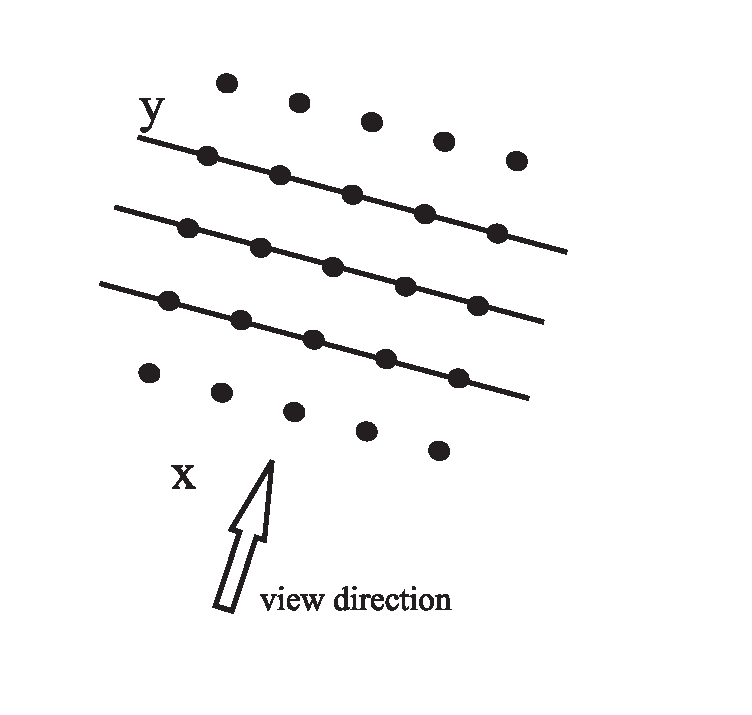
\includegraphics[width=2.0in]{figures/figDIRA2}&
\includegraphics[width=2.0in]{figures/figDIRA3}&
\includegraphics[width=2.0in]{figures/figDIRA1}\\
a) smoke planes parallel to $y$ axis& b) smoke planes parallel to
$y=x$ axis)&
c) smoke planes parallel to $x$ axis\\
\end{tabular}
\caption{View of smoke planes from above.  Smoke Planes are
oriented so that are {\em most perpendicular}\ to the line of sight }
\label{figDIRA}
\end{figure}

\begin{figure}
\centerline{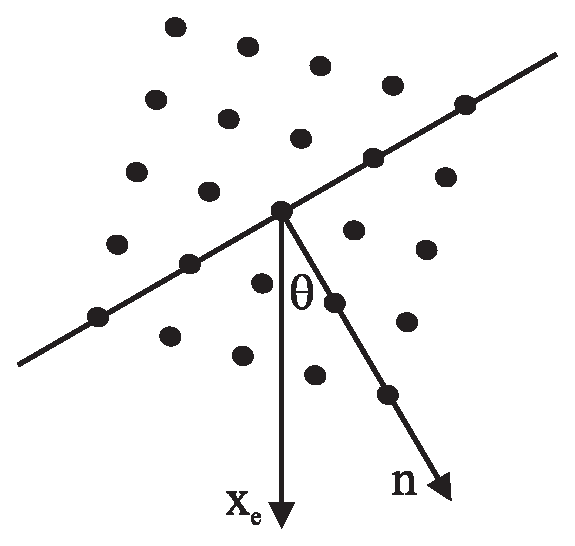
\includegraphics[width=3.0in]{figures/figDIRB}}
\caption{Diagram illustrating the angle between the line of sight
and smoke plane normal vector.  View planes are chosen to minimize
this angle.} \label{figDIRB}
\end{figure}
Smoke opacity data computed as described in previous sections is stored in a 3D array.
This array corresponds to the solution domain as setup in an FDS input file (or some other model).
Smoke planes are drawn in Smokeview through this data.  The orientation is chosen to be most perpendicular
to the viewers line of sight.  A plane orientation exactly perpendicular to the view direction could be drawn
if one is willing to pay the added CPU cost of interpolating opacity values between grid nodes.

Figure \ref{figDIRA} illustrates this process showing three view directions and the corresponding smoke plane orientations that would be used.
Off-axis viewing is minimized by selecting the view planes orientation that minimizes the angle between the planes normal direction and the view direction.
This angle, $\theta$, is illustrated in Figure \ref{figDIRB}, and is given by
\begin{eqnarray*}
\cos(\theta)=\frac{n\cdot v_e}{||n||||v_e||}
\end{eqnarray*}

\noindent where $n$ is normal vector for the candidate smoke plane, and $v_e$ is
the view direction vector.  In OpenGL, the view direction vector,
$v_e$, is computed by simply obtaining the modelview matrix, $M$
and multiplying it by the vector, $(0,0,1)^T$ or equivalently the
third row of $M$.


%................................
\part{Appendices}
\appendix
\chapter{Interfacing OpenGL with the Host Operating System}
OpenGL by design draws
the 3D geometry but does not interact with the user or the
operating system. Smokeview uses the graphics library utility
toolkit (GLUT) for interacting with the user {\em via}\ the
keyboard and mouse and for interacting with the operating system
to swap display buffers, to display fonts, to set maximum frame
rates {\em etc}. Though not as sophisticated as other libraries,
GLUT is simple to use and is portable allowing Smokeview to be
built on a number of different computer platforms including a PC
running Windows or Linux, a Silicon Graphics workstation running
IRIX or a Macintosh running OSX.

\section{Buffers} Smokeview uses several buffers provided by
OpenGL for visualization.  GLUT is used to manipulate these
buffers. Smokeview uses double buffering.  Double buffering is the technique where drawing occurs in the
{\bf back buffer}\ while the scene is simultaneously displayed using
the {\bf front buffer}. Smokeview uses the GLUT routine {\tt
glutSwapBuffers();}\ to swap the front and back buffers once
drawing is complete. Screen flickering occurs the if the display (front) buffer is updated while drawing occurs.

Hidden lines and surfaces are removed from a scene using the {\bf
depth buffer}.  Each time Smokeview draws an object, its depth
(distance from the observer) is compared to the value previously
stored in the depth buffer.  If the object's depth is less than
the value stored in the depth buffer then the object is considered
visible and the new depth value is store in the buffer. Otherwise
the depth buffer remains unchanged and the object is considered
hidden.

\section{Initialization and Callback Routines}
Initializations are performed by GLUT to set up windows and to
define display modes.  Smokeview defines the display to handle
color, a depth buffer and double buffering by passing the OpenGL
keywords {\tt GLUT\_RGB}, {\tt GLUT\_DEPTH} and {\tt GLUT\_DOUBLE}
to {\tt glutInitDisplayMode} as in

\begin{verbatim}
  glutInitDisplayMode(GLUT_RGB|GLUT_DEPTH|GLUT_DOUBLE);
\end{verbatim}

Smokeview creates a window with width {\tt windW}\ and height {\tt
windH} using the GLUT calls

\begin{verbatim}
  glutInitWindowSize(windW, windH);
  glutCreateWindow("");
\end{verbatim}

and defines callbacks with

\begin{verbatim}
  glutSpecialUpFunc(specialkeyboard_up);
  glutKeyboardUpFunc(keyboard_up);
  glutKeyboardFunc(keyboard);
  glutMouseFunc(mouse);
  glutSpecialFunc(specialkeyboard);
  glutMotionFunc(motion);
  glutReshapeFunc(Reshape);
  glutDisplayFunc(Display);
\end{verbatim}

A callback is a routine that is called when a particular event
occurs.  For Smokeview these events would be when a keyboard key
is depressed (or when the key is released), when the mouse is
clicked or when the mouse is moved.  Smokeview determines rotation
and translation amounts using the {\tt motion} callback defined
with {\tt glutMotionFunc(motion)}.

\chapter{Compressing Data}
\chapter{Rendering Smokeview Images}

Smokeview uses the library GD\cite{GDLIB} to convert the currently displayed scene into either a JPEG, PNG or GIF image.  Smokeview reads in the OpenGL back buffer and then uses the GD routine, {\tt gdImageSetPixel}\ to store the image data in GD's internal format one pixel at a time.    Finally, Smokeview uses a GD routine to convert the image into the desired image format.

A summary of the steps in more detail are:
\begin{enumerate}
\item Allocate memory buffers and file pointers
\begin{verbatim}
  RENDERfile = fopen(RENDERfilename, "wb");
  pixels = (GLubyte *) malloc(width * height * sizeof(GLubyte) * 3);
\end{verbatim}

\item Read pixel data from the back buffer
\begin{verbatim}

  glReadPixels(x, y, width, height, GL_RGB, GL_UNSIGNED_BYTE, OpenGLimage);
\end{verbatim}
\item ALlocate the gd data structures used to hold image data
\begin{verbatim}
  RENDERimage = gdImageCreateTrueColor(width,height);
\end{verbatim}

\item Set pixel data

\begin{verbatim}
  for (i = height-1 ; i>=0; i--) {
    for(j=0;j<width;j++){
      r=*p++; g=*p++; b=*p++;
      rgb = (r<<16)|(g<<8)|b;
      gdImageSetPixel(RENDERimage,j,i,rgb);

    }
  }
\end{verbatim}

\item Write out data to a JPEG image file

\begin{verbatim}
    gdImageJpeg(RENDERimage,RENDERfile,-1);
\end{verbatim}

\item deallocate memory buffers and free file pointer

\begin{verbatim}
  fclose(RENDERfile);
  gdImageDestroy(RENDERimage);
  free(OpenGLimage);
\end{verbatim}

\end{enumerate}







\bibliography{../Bibliography/FDS_refs,../Bibliography/FDS_mathcomp,../Bibliography/sv_fire,../Bibliography/sv_graphics}

\addcontentsline{toc}{chapter}{References}

%\appendix
%\addcontentsline{toc}{chapter}{Appendices}


\end{document}
